\chapter{Introdução}

Com o aumento da popularidade da internet em todo o mundo, é notável que as redes WiFi têm crescido significativamente, juntamente com o número de usuários e de dispositivos IoT (Internet Of Things). De acordo com o relatório Digital 2023: Global Overview Report, publicado pelo site Datareportal, há cerca de 5,16 bilhões de usuários da internet atualmente. No entanto, esse aumento na demanda por WiFi tem causado um problema, que é a congestão das faixas do espectro eletromagnético reservadas para essas redes, assim afetando a sua eficiência.

\begin{figure}[htb]
  \centering
  \caption{Indicadores de uso da Internet}
  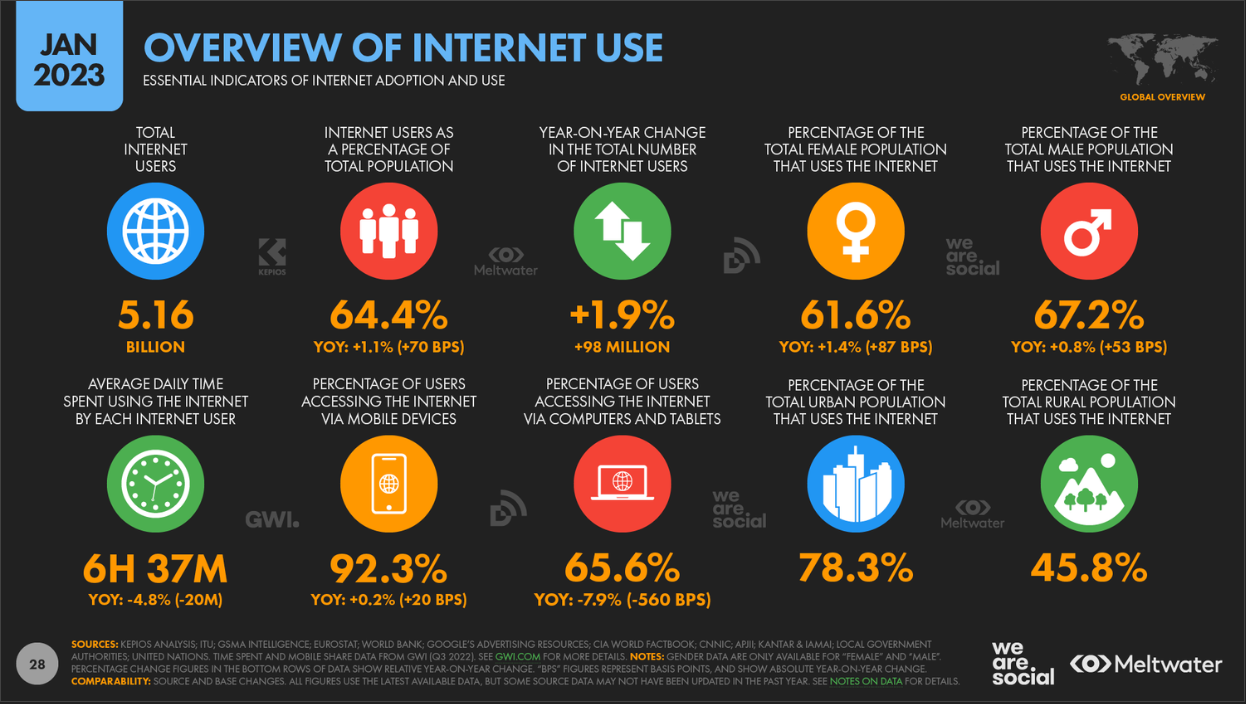
\includegraphics[scale=0.45]{images/internet_use.png}
  \legend{Fonte: \citeonline{Datareportal}}
  \label{figura:usoInternet}
\end{figure}

As redes  wireless utilizam ondas eletromagnéticas para a transmissão de dados e informações, o que inviabiliza ou dificulta a sua utilização em alguns lugares, como em hospitais e aeronaves, por exemplo, por interferir com equipamentos hospitalares e com a antena de transmissão no caso dos voos.

Se deparando com esses cenários, o Visible Light Communication (VLC) se mostra como um forte candidato para a solução destes problemas. Pois percebemos que o espectro da luz visível, possui 10 mil vezes mais faixas de frequência se comparado com as ondas de rádio, \citeonline[p. 14]{conceiccao2015comunicaccao}. Ou seja, é possível que um único “roteador” se comunique com mais dispositivos ao mesmo tempo.

Para o problema de interferência o VLC também é uma solução, visto que utiliza a luz visível como forma de transmitir as informações, assim não gerando interferências eletromagnéticas em outros aparelhos eletrônicos ou em redes wifi.

Assim, o estudo objetiva verificar a viabilidade de implementação do sistema VLC com o mini-computador Raspberry Pi, através da construção de um protótipo. A pesquisa experimental surgiu da necessidade de uma nova forma de transmissão de dados com pouca interferência e de baixo custo. Abrindo uma  possibilidade de levar comunicação em locais onde não era possível recorrer a uma rede wireless.

